% !TEX root = 1_Main.tex

\begin{block}{Common tools}
\vskip-2ex
  \begin{columns}[t]\hfill\hfill\hfill
    \begin{column}{.45\linewidth}
 \begin{subblock}{\faIcon{folder} \hfill Data and File Organization\hfill \faIcon{folder-open}}
%TIER protocol \href{https://www.projecttier.org/tier-protocol/protocol-4-0/}{ProjectTIER.org}

Research Data Alliance \href{rd-alliance.org/}{rd-alliance.org/}
    \vskip-1ex
  \end{subblock}
  
  \begin{subblock}{\faDatabase \hfill Data Repositories \hfill \faDatabase}
 \begin{itemize}
     \item \textbf{Open Science Framework (OSF)}
     \item Zenodo
     \item Harvard Dataverse
     \item ICPSR
    %  \item Dryad
    %  \item Figshare
    %  \item Vivli

 \end{itemize}
    \vskip-1ex
  \end{subblock}
  
  \begin{subblock}{\faIcon{table} \hfill Paper Repositories \hfill \faIcon{table}}
 \begin{itemize}
     \item \textbf{Open Science Framework (OSF)}
     \item arXiv
 \end{itemize}
    \vskip-1ex
  \end{subblock}  

  \begin{subblock}{\faSearch \hfill Make your work findable\hfill \faSearch}
Ensure it is indexed and has a unique identifier. Try CrossRef, ORCiD, doi.

    \vskip-1ex
  \end{subblock}  
  
  \begin{subblock}{\faIcon{id-badge}\hfill Licenses\hfill \faIcon{id-badge}}
 \begin{itemize}
\item CC-BY \href{https://creativecommons.org/about/cclicenses/ 
}{creativecommons.org}
\item MIT \href{https://mit-license.org/ }{mit-license.org}
 \end{itemize}
    \vskip-1ex
  \end{subblock}  

  \end{column}\hfill
   \begin{column}{.45\linewidth}

\begin{subblock}{\faIcon{file-alt} \hfill Analysis tools\hfill \faIcon{file-alt}}
Open source software is more transparent \\ \vspace{0.5em}
 \faIcon{r-project} R \href{https://www.r-project.org/}{r-project.org}
\\ \faIcon{python} Python \href{https://www.python.org/}{python.org}
\\ JASP \href{https://jasp-stats.org/}{jasp-stats.org} \\ \vspace{0.5em}
...but, you can be transparent with closed-source software, too!
  \end{subblock}
   
\begin{subblock}{\faIcon{file-alt}\hfill Literate programming\hfill \faIcon{file-alt}}
Mixing text and code helps document your work \\ \vspace{0.5em} \faIcon{r-project}, \faIcon{python}, \faIcon{file-code}  Quarto \href{https://quarto.org/}{quarto.org}
\\ \faIcon{r-project} RMarkdown \href{https://rmarkdown.rstudio.com/}{rmarkdown.rstudio.com}
\\ \faIcon{python} Jupyter Notebooks \href{https://jupyter.org/
}{jupyter.org}
  \end{subblock}

  \begin{subblock}{\faIcon{file-code}\hfill Code Repositories\hfill \faIcon{file-code}}
\begin{itemize}
    \item GitHub \faIcon{github}
    %\item Open Science Framework (OSF)
    \item Zenodo
    \item GitLab \faIcon{gitlab}
    \item Bitbucket \faIcon{bitbucket}

\end{itemize}
  \end{subblock}
  \end{column}\hfill\hfill\hfill

  \end{columns}
   ...there are many more resources in all these categories! Pull requests welcome.   
   
% \begin{center}
%     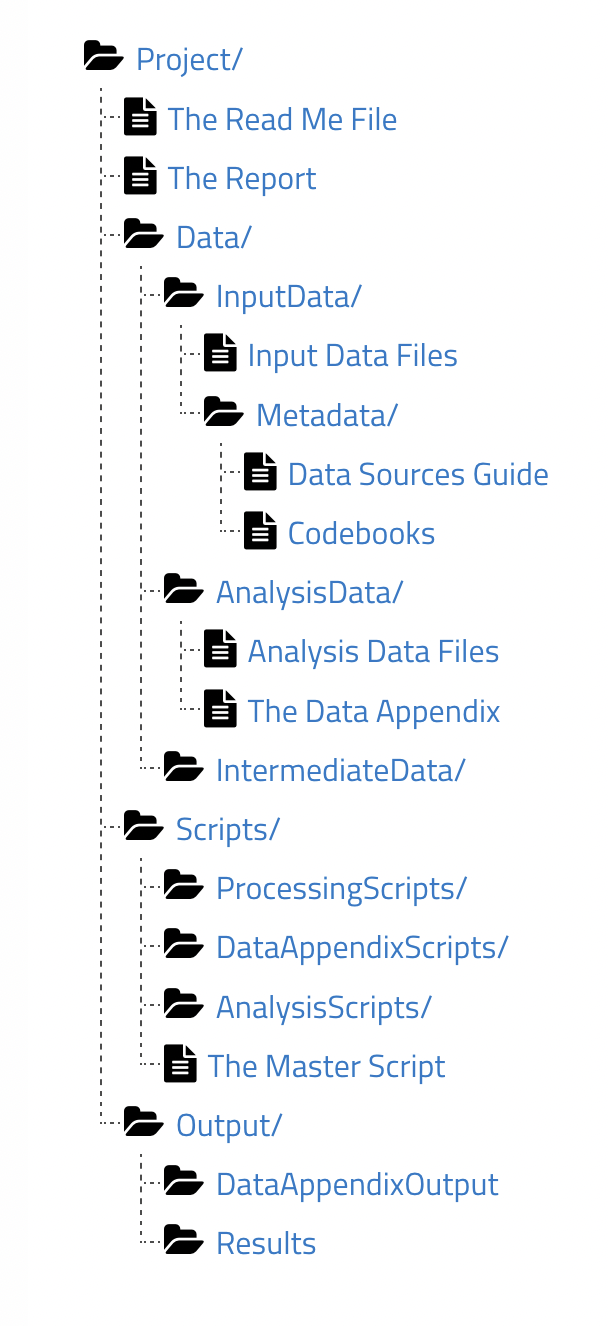
\includegraphics[width=0.6\textwidth]{img/TIER_protocol.png} \\
%     TIER Protocol ProjectTIER.org
% \end{center}

\end{block}